\chapter{Work Object Data}
\label{ch:workobject}
\markboth{Work Object Data}{}

\begin{flushright}
	{\smaller
		\textit{It is not certain\\ that everything is uncertain}\\
		-- Blaise Pascal}
\end{flushright}

All the following analysis will be carried out using a default aircraft. This choice is made in order to avoid the collection and validation data phase for each analysis and make focus on the results. As mentioned, there are two default aircraft in the code: ATR-72 and Boieng 747\_100B whose data are shown in the table below.\\
All the analysis that follow, refer to the data presented in this chapter and those derived from them .

\begin{figure}[H]
\centering
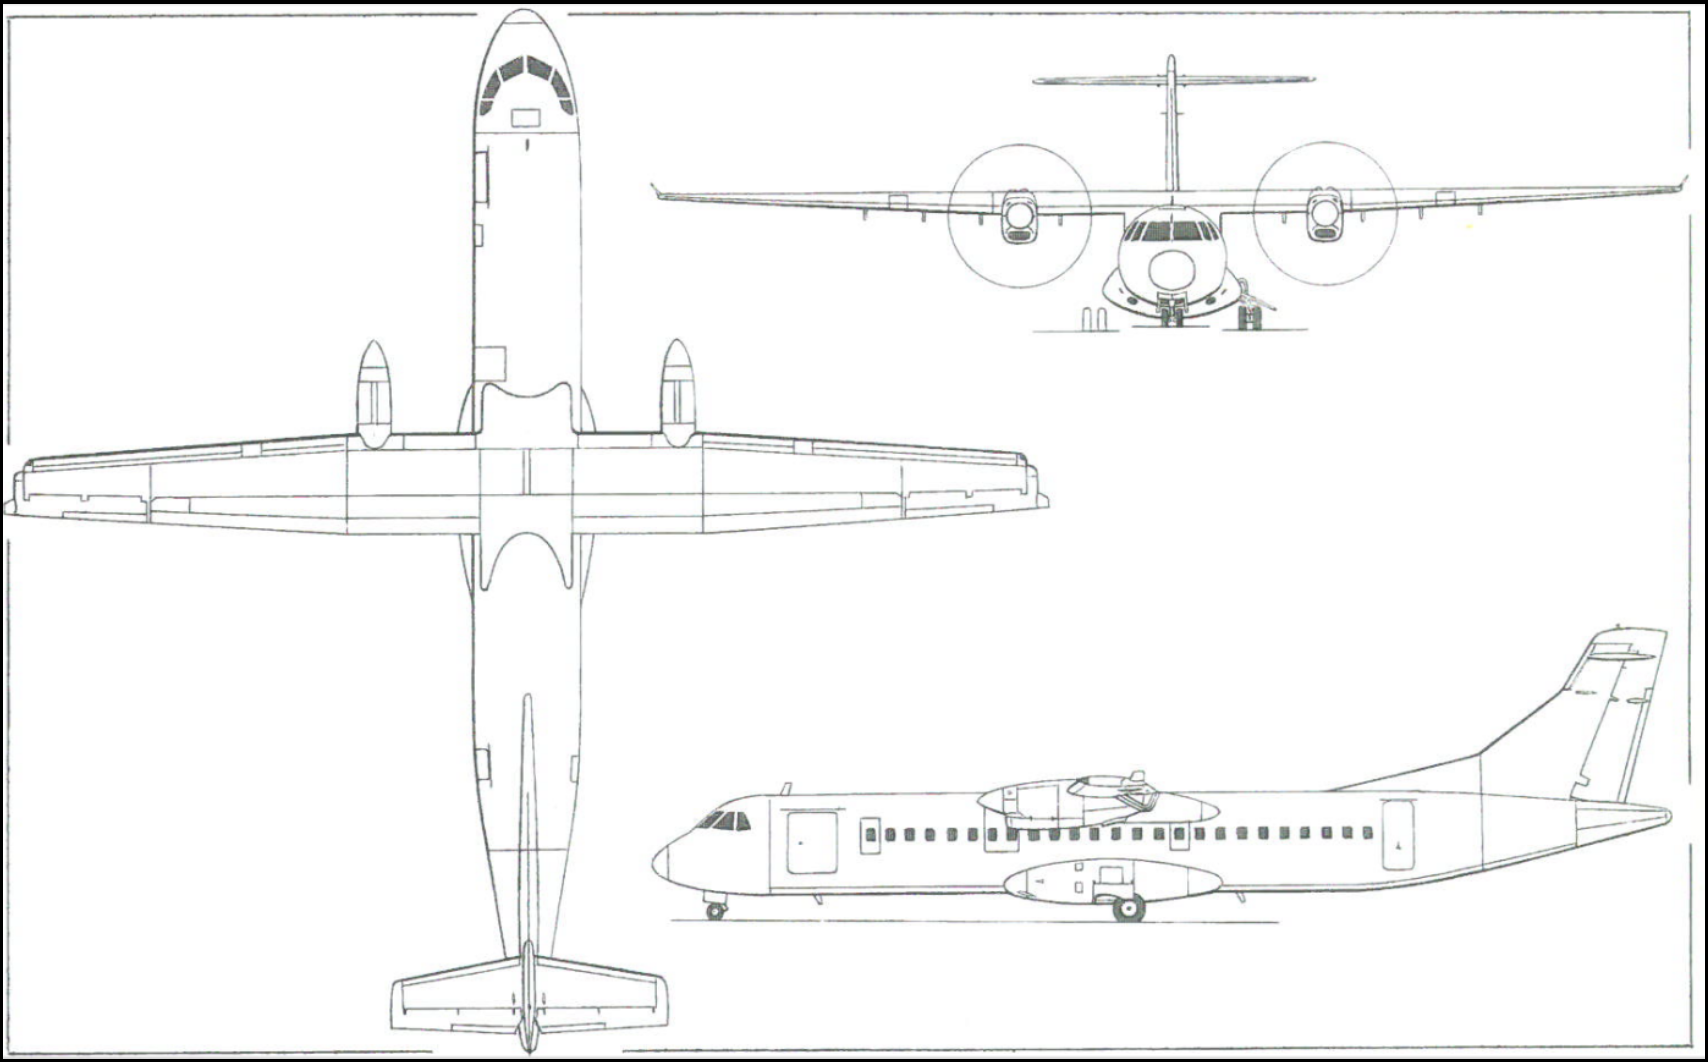
\includegraphics[height=6.4cm]{Immagini/ATR-72}
\caption{ATR-72 views – Jane’s All the World’s Aircraft 2004-2005.}
\label{atr}
\end{figure}
\begin{figure}[H]
\centering
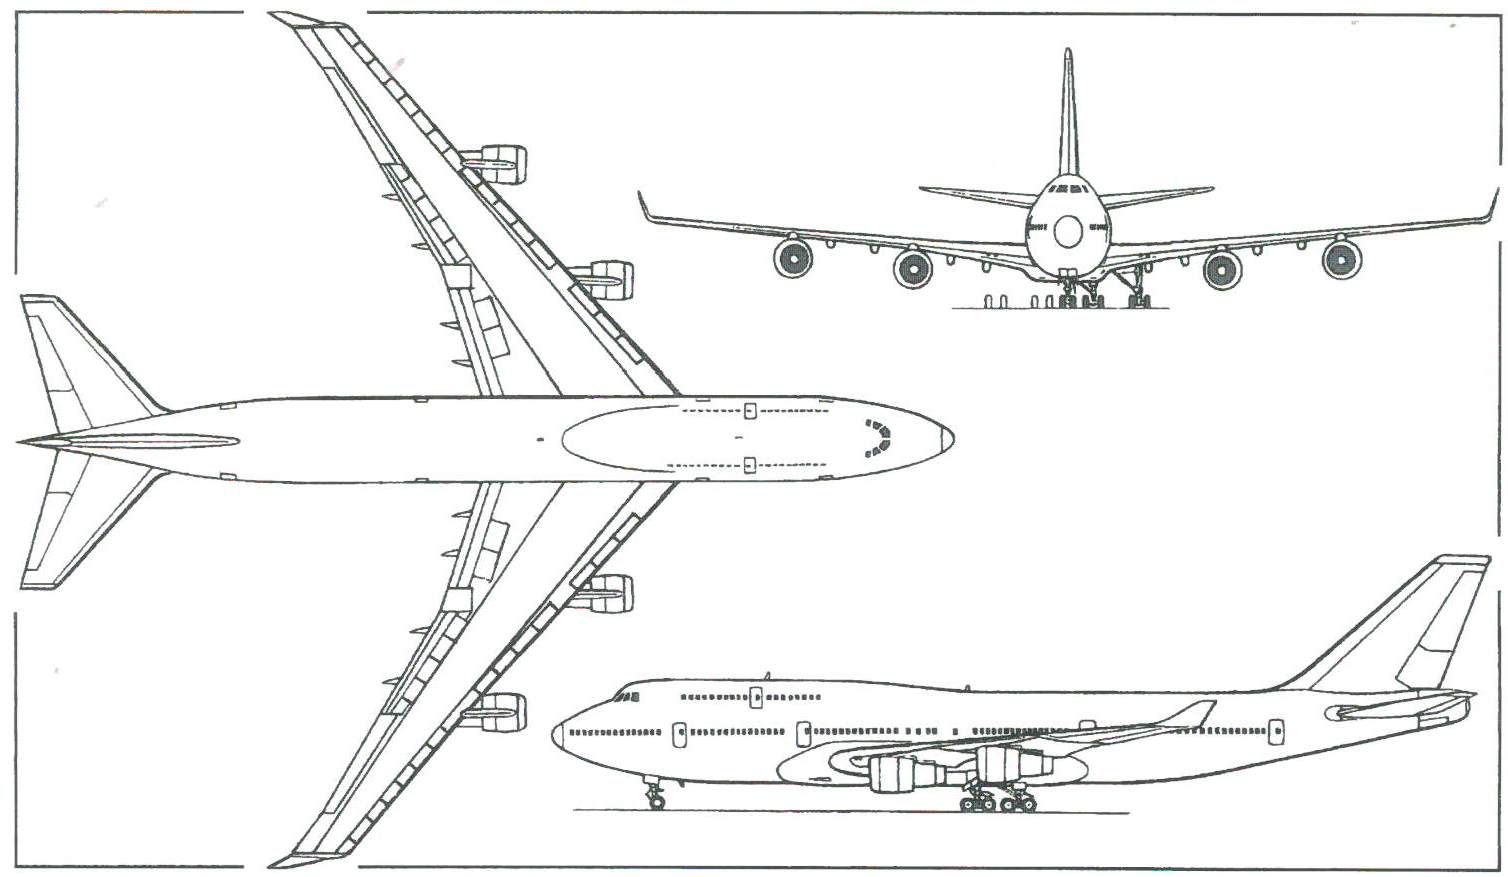
\includegraphics[height=6.4cm]{Immagini/B747-100B}
\caption{B747-100B views – Jane’s All the World’s Aircraft 2004-2005.}
\label{boeing}
\end{figure}